\chapter{Voraussetzungen}
	
	\section{RESTful APIs} % Raphael
	
		Representational State Transfer beschreibt ein architektonisches Modell, um Web Services zu erstellen. Sogenannte \acs{REST} Web Services bieten Interoperabilität zwischen Computersystemen im Internet -- geeignet für die Kommunikation von Maschine zu Maschine. So lässt sich REST auch als eine Abstraktion der Struktur und des Verhaltens des World Wide Webs beschreiben. 
		
		Neben REST gibt es weitere Alternativen, wie \acs{SOAP} oder \acs{RPC}; der Vorteil von REST besteht jedoch darin, dass durch das \acs{WWW} ein Großteil der Infrastruktur für die Kommunikation bereits vorhanden und implementiert ist. Während bei \\acs{RPC} in der \acs{URI} Methodeninformationen enthalten sind, gibt eine \acs{URI} in der \acs{REST} Architektur ausschließlich Ressourcen an und kodiert die Funktionalität mittels \acs{HTTP} Methoden. Dieser Ansatz entspricht dem Konzept einer \acs{URI}, da bei einer \acs{HTTP} Anfrage ebenso nur Ressourcen und keine Funktionalität gefragt ist.
		
		Eine REST API muss insgesamt sechs Eigenschaften besitzen:
		
		\begin{description}
			\item[Client-Server Architektur] 
				Bei \acs{REST} gilt im Allgemeinen, dass eine Client-Server Architektur vorliegen soll: Der Client konsumiert die vom Server bereitgestellten Dienste. 
			\item[Zustandslosigkeit] 
				Eine RESTful \acs{API} hat keine Zustände, sondern ist so konzipiert, dass benötigten Informationen in einer REST-Nachricht enthalten sind. Dies begünstigt außerdem die Skalierbarkeit eines solchen Dienstes, da es auf diese Weise einfacher ist, alle eingehenden Anfragen auf mehrere Instanzen zu verteilen.
			\item[Caching] 
				Server sowie Client können Antworten zwischenspeichern. Es muss jedoch vorher explizit definiert werden, welche Antworten zwischengespeichert und welche nicht zwischengespeichert werden, um zu verhindern, dass alte oder ungeeignete Daten versendet werden.
			\item[Einheitliche Schnittstelle]
				Die \acs{REST} \acs{API} muss eine einheitliche Schnittstelle zur Verfügung stellen, welche den von \cite{RoyThomasFielding.2000} definierten Anforderungen entsprechen muss. Dies vereinfacht die Nutzung der \acs{API}.
			\item[Mehrschichtige Systeme]
				 Die Struktur einer RESTful \acs{API} soll mehrschichtig sein, sodass es ausreicht, dem Client lediglich die oberste Schicht als Schnittstelle anzubieten. Die Architektur der API wird dadurch simplifiziert und die dahinterliegenden Schichten der Implementierung bleiben verborgen.
			\item[Code on Demand] 
				Fielding beschreibt diese Eigenschaft als optional: Der Server kann, durch das Übertragen von ausführbarem Code, die Funktionalität des Clients zeitweise erweitern oder anpassen. Vorstellbar wäre beispielsweise eine Übertragung von bereits kompilierten Komponenten oder Client-seitigen Skripten. Dies gilt es jedoch mit Vorsicht zu genießen, da diese Funktionalität auch Sicherheitslücken bergen und somit eine geeignete Angriffsmöglichkeit bieten kann. 
				
		\end{description}

	\section{Frameworks}
	
		\subsection{OpenAPI} % Raphael
		
			Der OpenAPI Standard ist Open Source und dient der Beschreibung von RESTful APIs. Bis 2016 war OpenAPI Teil des Swagger Frameworks, wurde aber schließlich als separates Projekt unter Aufsicht der sog. \textit{OpenAPI Initiative}  ausgelagert. 
			
			Mit der deklarativen Ressourcenspezifikation von OpenAPI können Clients Dienste verstehen und konsumieren, ohne über Kenntnisse der eigentlichen Server-Implementierung bzw. Zugriff auf den Servercode zu verfügen. Dies erleichtert die Entwicklung Client-seitiger Applikationen, die RESTful APIs verwenden. Die OpenAPI-Spezifikation ist zudem sprachunabhängig und lässt sich in jeder Beschreibungssprache (\acs{YAML}, \acs{XML} etc.) definieren. 
			
			Zu dieser Spezifikation der API gehören unter anderem folgende Metadaten:
			
			\begin{itemize}
				\item Name der API
				\item Version
				\item Kurzbeschreibung
				\item Kontakt
				\item Lizenz
			\end{itemize}
		
			Wichtig ist hierbei vor allem die Version. Diese ermöglicht es, auch auf ältere Versionen der \acs{API} zuzugreifen, sodass nach einem Update, nicht jeder Konsument dieser \acs{API} zum einen die Version ändern und zum anderem eventuell auch Code anpassen muss.
			
			Darüber hinaus lassen sich Schemata beschreiben, die das Datenmodell für Konsumenten repräsentieren. Diese Schemata sind mittels der \acs{JSON} Schema Specification definiert. Es können verschiedene Objekte definiert werden, die mehrere Attribute mit einem definierten Datentypen haben. Dieser Datentyp kann wiederum ein Schema eines Objektes sein, sodass eine Verschachtelung von Objekten möglich ist. \cite{.2252020}
			
			Der Hauptteil der API Beschreibung entspricht der Definition der eigentlichen Schnittstelle. Hierbei können Pfade definiert werden, welche die API öffentlich zur Verfügung stellt. Pro Pfad -- bzw. Ressource -- lassen sich die möglichen \acs{HTTP} Operationen definieren. Diese Definition beinhaltet die geforderten Parameter und möglichen Rückgabewerte bzw. -codes inkl. einer Beschreibung. Bei einer erfolgreichen Anfrage können die bereits definierten Schemata verwendet werden, um den Rückgabetyp zu definieren. So lassen sich alle möglichen Anfragen an die \acs{API} klar definieren, sodass inkorrekte Anfragen nicht zugelassen werden.
			
			Die definierten Pfade lassen sich zudem in Tags zusammenfassen, sodass eine gewisse Struktur in den Anfragen gewährleistet und außerdem die Komplexität der \acs{API} reduziert wird. 
	
		\subsection{Swagger} % Raphael
		
			Swagger ist ein Framework, das sich des OpenAPI Standards bedient. Swagger bietet ein Tooling an, mit dessen Hilfe \acs{API}s spezifiziert und beschrieben werden können. Neben einem entsprechenden Editor, bietet Swagger die Möglichkeit, aus der OpenAPI Spezifikation Code zu generieren und zwar unter Verwendung unterschiedlicher Frameworks -- z.B. eine vollständige Spring Applikation --, wobei nur noch die eigentliche Implementierung der Businesslogik erforderlich ist.
			
			Des Weiteren stellt Swagger eine Web-basierte Benutzeroberfläche zur Verfügung, welche nicht nur die direkte Anbindung von Live \acs{API}s ermöglicht, sondern auch eine visuelle Dokumentation der \acs{API} darstellt. \cite{SmartBear.2020}
			
			Swagger stellt zudem die Plattform SwaggerHub öffentlich zur Verfügung. Auf dieser Plattform können \acs{API} Spezifikationen veröffentlicht werden. Somit sind die Spezifikationen vieler verschiedener \acs{API}s auf einer Plattform zusammengefasst und können einfach eingesehen werden. \autoref{fig:swaggerHub} zeigt die Darstellung der Plattform SwaggerHub.
			
			\begin{figure}[ht!]
				\centering
				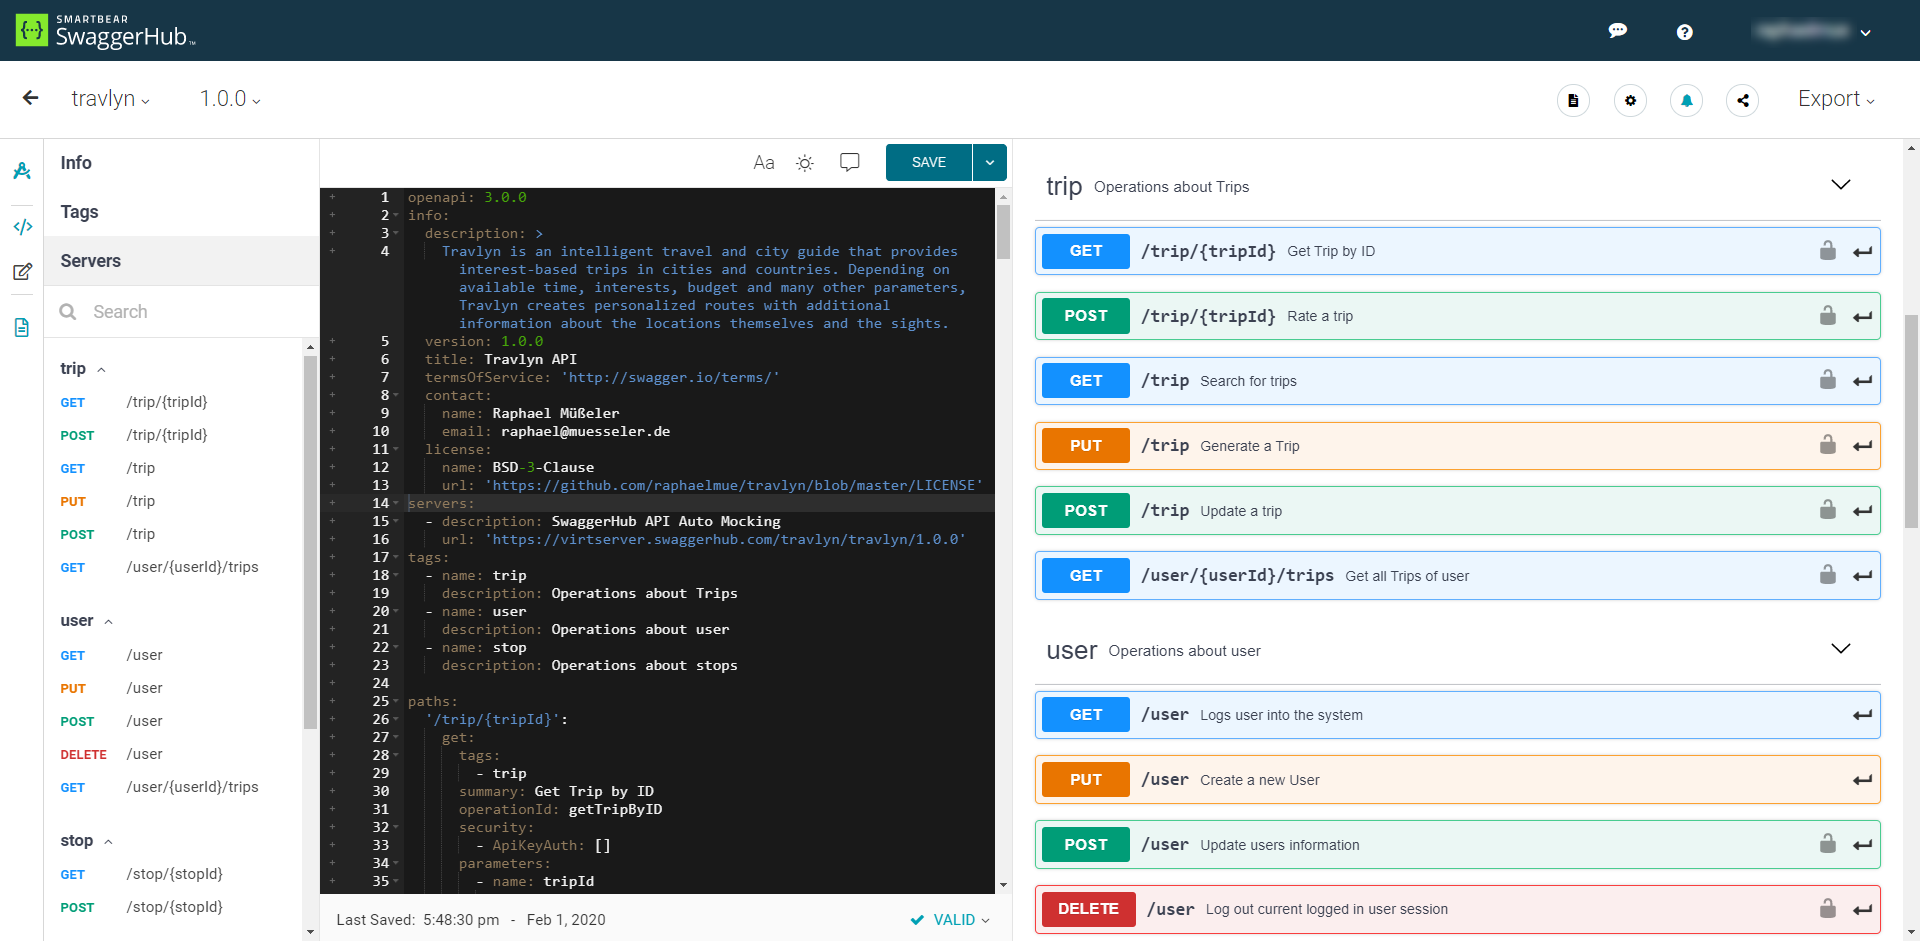
\includegraphics[width=1\textwidth]{images/swagger-hub.png}
				\caption{SwaggerHub Darstellung anhand des Projektes \textit{Travlyn}}
				\label{fig:swaggerHub}
			\end{figure} 
			
		\subsection{Spring} % Raphael
		
			Spring ist ein Open Source Framework, welches in Java geschrieben wurde. Es gilt als de facto Standard bei der Entwicklung von RESTful API, da es in der Open Source Welt viel Zuspruch und Verwendung gefunden hat. Zudem integriert Spring mit fast allen Java Umgebungen und ist somit nicht nur für Anwendungen im kleinen Maßstab, sondern eben so für Anwendungen in großen Unternehmen geeignet. \cite{Walls.20162017} 
			
			Bei der Entwicklung dieses Frameworks wurden die unter anderem in \cite{Johnson.2003} beschriebenen Design Prinzipien mithilfe der folgenden Module und deren entsprechender Funktionalität umgesetzt:
			
			\subsubsection{Dependency Injection} % Raphael
			
				Der von Martin Fowler 2004 definierte Begriff der \textit{Dependency Injection} in \cite{MartinFowler.23.01.2020} ist eine Präzisierung oder Spezialisierung des Begriffs \textit{Inversion of Control}. \acs{IoC} bezeichnet ein Paradigma, welches den Kontrollfluss einer Applikation nicht mehr der Anwendung, sondern dem Framework -- in diesem Fall Spring -- überlässt. Ein Beispiel für \acs{IoC} sind Listener (Beobachter Muster). \\
				Dependency Injection beschreibt ein Entwurfsmuster, bei welchem festgelegte Abhängigkeiten nicht zur Kompilierzeit, sondern zur Laufzeit bereitgestellt werden. Dies lässt sich einem Beispiel erläutern: Besteht bei der Initialisierung eines Objektes eine Abhängigkeit zu einem anderen Objekt, so wird diese Abhängigkeit an einem zentralen Ort hinterlegt. Wenn nun die Initialisierung dieses Objektes erfolgt, beauftragt es den sog. Injector (dt. Injezierer), die Abhängigkeit aufzulösen. \cite{MartinFowler.23.01.2020}
				
				In Spring bietet der \acs{IoC} Container mittels Reflexion ein konsistentes Werkzeug zur Konfiguration sowie Verwaltung von Java Objekten. Diese durch den Container erstellten Objekten heißen \textit{Beans}. Die Konfiguration des Containers erfolgt entweder über eine \acs{XML} Datei oder über Java Annotationen. \cite{Walls.20162017} 
				
			\subsubsection{Aspektorientierte Programmierung}
			
				\acs{AOP} beschreibt ein Paradigma und ermöglicht die klassenübergreifende Verwendung generischer Funktionalität. Dies führt zu einer starken Modularisierung und sorgt für eine klare Trennung zwischen der Anwendungslogik und der Businesslogik (Cross-cutting Concern). \cite{Wunderlich.2005} \\
				Das Schreiben von Logs stellt ein Beispiel für ein Cross-cutting Concern dar, da eine Logging-Strategie alle protokollierten Klassen und Methoden erfasst und somit durchaus mit der Anwendungs- sowie der Businesslogik in Berührung kommt. 
			
			\subsubsection{Transaktionsmanagement} % Raphael
			\label{frameworks.spring.transaktionsmanagement}
			
				Ein weiteres Beispiel für \acs{AOP} ist sog. Transaktionsmanagement. Eine Transaktion bezeichnet in der Informatik eine logische Einheit, mit dessen Hilfe Aktionen auf einer Persistenz ausgeführt werden können. Dabei ist sichergestellt, dass sobald die Transaktion fehlerfrei und vollständig abgeschlossen ist, der Datenbestand weiterhin konsistent ist. Im Umkehrschluss bedeutet das, dass eine Transaktion entweder vollständig oder gar nicht ausgeführt wird. \cite{Ozsu.2011}
			
				Das von Spring bereitgestellte Transaktionsmanagement stellt eine Abstraktion der Java Plattform dar und ist in der Lage mit globalen und verschachtelten Transaktionen sowie sog. Savepoints -- ein Punkt innerhalb einer Transaktion, zu welchem im Fehlerfall zurück gesprungen werden kann -- zu arbeiten. Außerdem lasst sich diese Abstraktion in fast allen Java Umgebungen einsetzen. Die von Java bereitgestellte Java Transaction API (\acs{JTA}) hingegen unterstützt nur globale und verschachtelte Transaktionen und erfordert zudem immer einen Applikationsserver. 
			
			\subsubsection{Model View Controller} % Raphael
			
				Das \acs{MVC} (Model View Controller) Pattern ist ein weit verbreiteter Mechanismus zur Entwicklung von Benutzeroberflächen. \acs{MVC} stellt ein Design Pattern dar, dass Kapselung sowie eine Struktur für eine Architektur von Benutzeroberflächen bietet und bei welcher jeder Bereich eine definierte Aufgabe hat. Eine Verletzung der Zuständigkeitsbereiche ist zu vermeiden. \cite{Gamma.1995}
			
				Das Pattern besagt, dass die Architektur von Benutzerschnittstellen in folgende Bereiche aufgeteilt ist: Das \textit{Model} ist für den Zugriff auf die Datenbank und die Beschaffung von Daten zuständig. Häufig ist das Model auch für die Aufbereitung der Daten zuständig. Somit liegt die meist aufwändige Logik nicht beim Client, sondern bei den Servern, welche zumeist auch mit besserer Hardware ausgestattet sind. \\
				Ein \textit{Controller} definiert die Art und Weise, wie die Benutzerschnittstelle auf die Eingaben des Benutzer reagiert. Des Weiteren ist ein Controller für das Aktualisieren der Daten im Datenmodell, aber auch auf dem View zuständig. \\
				Der \textit{View} bestimmt ausschließlich, wie die Benutzeroberfläche aussehen soll. Er enthält -- in den meisten Implementierungen -- keine Logik, sondern ist lediglich eine Definition und Anordnung der Benutzeroberflächenelemente.
				
				Spring definiert für alle Verantwortlichkeiten eigene Strategie-Interfaces, wie beispielsweise das Controller Interface, welches alle eingehenden \acs{HTTP} Requests definiert und darüber hinaus auch behandelt. 

		
		\subsection{Hibernate} % Raphael
		
			Hibernate ist ein Persistenz- und Object-relational Mapping (\acs{ORM}) Framework, das ebenfalls unter einer Open Source Lizenz veröffentlicht und in Java geschrieben ist. Hibernate bietet eine Abstraktionsstufe gegenüber relationalen Datenbankimplementationen. Mithilfe der Sprache \textit{Hibernate Query Language} und dem entsprechend konfigurierten Dialekt (z.B. MySQL Dialekt, MariaDB Dialekt etc.) werden die entsprechenden Statements erzeugt und schließlich ausgeführt. Dies ermöglicht den einfach und schnellen Umstieg von einer Datenbankimplementation auf die andere, ohne Anpassung der sich im Code befindlichen Queries. 
			
			\subsubsection{Object-relational Mapping} % Raphael
		
				Eine häufig eingesetzt Technik der Persistierung sind relationale und meist auch \acs{SQL} basierte Datenbanken wie beispielsweise MySQL oder MariaDB. Wenn jedoch die Anwendung, welche die Businesslogik enthält, der Objektorientierung folgt, kommt es zu einem Widerspruch -- dem sog. \textit{Object-relational impedance mismatch} --, welcher in den unterschiedlichen Paradigmen begründet liegt. So beschreibt die Objektrelationale Abbildung eine Technik, bei welcher sich Objekte einer objektorientierten Sprache in einer relationalen Datenbank persistieren lassen. \cite{Ireland.2009}
					
				Java bietet mit der sog. Java Persistence API (\acs{JPA}) eine Abstraktion genau zu diesem Zweck, dessen sich Hibernate auch bedient. Mittels Annotationen lassen sich Objekte mit Attributen und Methoden -- zumeist Plain Old Java Objects (\acs{POJO}s) -- auf Entitäten abbilden. Diese Annotation definieren, welche Tabelle auf welches Objekt und welche Spalte auf welches Attribute abgebildet wird. Es lassen sich außerdem die Relationen der Entitäten auf die Assoziationen der Objekte abbilden. Hibernate bzw. \acs{JPA} unterstützt 1:1, 1:N sowie N:N Relationen. Somit wird ein vollständiges Abbild der Persistenz in der Anwendung geschaffen.
				
				Die einzige Vorgabe bei der Definition der Objekte ist, dass ein parameterloser Konstruktor existieren muss. Hibernate greift auf die Attribute der Klasse mittels Reflexion zu. 
				
			\subsubsection{Transaktionsmanagement} % Raphael
			
				In Hibernate erfolgt der Zugriff auf die Persistenz über sogenannte \textit{Sessions}. Eine Session repräsentiert eine physische Verbindung zwischen der Persistenz und der Anwendung und bietet Methoden für alle Datenbestandsoperationen. Der Lebenszyklus einer \textit{Session} ist durch den Beginn und das Ende einer logischen Transaktion begrenzt. Es ist konfigurierbar, ob Hibernate das Sessionmanagement übernimmt, oder die Anwendung selbst die \textit{Sessions} öffnet und wieder schließt. So werden auch parallele Datenbankverbindung und damit auch eine Performance Verbesserung ermöglicht.
				
				Um eine Session mittels des Sessionmanagements zu erstellt, wird sich der \textit{SessionFactory} bedient, von welcher meist nur eine Instanz in der Applikation existiert. Diese beinhaltet die Konfiguration, die den Verbindungsaufbau und die Verbindung selbst definiert.
				
				Eine Session ermöglicht es eine \textit{Transaction} -- Abstraktion der Implementation von \acs{JTA} -- zu starten und zu beenden. Wie bereits in \autoref{frameworks.spring.transaktionsmanagement} beschrieben, lässt sich hierbei das Transaktionsmanagement sehr gut integrieren, sodass Spring das Starten und Beenden von Transaktionen handhabt. Dies führt zu einer Simplifizierung des Codes, der zum einen lesbarer und zum anderen einfacher wird. 
				
		\subsection{Docker} % Raphael
			
			Docker ist eine Open Source Virtualisierungssoftware, die der Isolierung von Anwendungen dient und von Docker Inc. bereitgestellt wird. Die Motivation hinter der Verwendung von Docker liegt im Deployment Prozess begründet: 
			
			Der noch vor einigen Jahren vorherrschende Auslieferungsprozess war zumeist eine Installationsanleitung, welche die einzelnen Anweisungsschritte beinhaltete, die es auszuführen galt, um die Applikation zu starten. Da dies jedoch auf Dauer zu komplex wurde, wurden Anwendungen mittels virtueller Maschinen ausgeliefert. Hierbei bestand der Vorteil darin, dass keine Abhängigkeiten o.Ä. installiert, sondern lediglich die virtuelle Maschine mit dem ausgelieferten Image gestartet werden musste. Jedoch beinhaltet ein solches Image ein vollständiges Gastbetriebssystem, dessen Größe die der Anwendung um einiges überstieg und damit nicht effizient und geeignet war. Des Weiteren stellt die Dauer des Starts einer virtuellen Maschine auch ein Problem dar. \\
			Um nun all diesen Problemen entgegenzuwirken, wurde Docker ins Leben gerufen. So werden alle Abhängigkeiten einer Anwendung in einem sog. Docker Image zusammengefasst, aus welchem wiederum Instanzen -- sog. Docker Container -- erzeugt werden. Diese leichtgewichtigen Images können nun sehr einfach ausgeliefert werden und sind darüber hinaus in der Lage, sehr schnell zu starten. \cite{ThomasClaudiusHuber.2019}
			
			Der Unterschied zwischen Docker und einer virtuellen Maschine besteht darin, dass, anstelle eines vollständigen Gastsystems, ein Docker Container sich des Betriebssystems des Hosts bedient, dem sog. Host OS. Mittels der Docker Engine wird der Zugriff auf den Kernel des Betriebssystems sichergestellt und diese bietet zudem die Möglichkeit Container zu erstellen, zu stoppen oder zu starten. \autoref{fig:dockerComparison} stellt diesen Unterschied graphisch dar. \cite{Turnbull.2014}
			
			\begin{figure}[ht!]
				\centering
				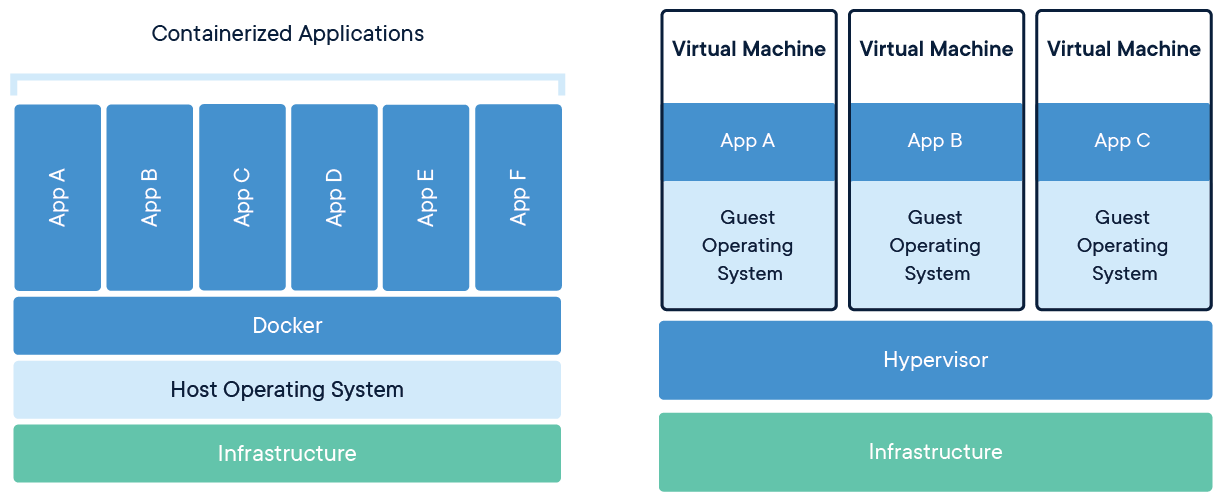
\includegraphics[width=1\textwidth]{images/docker-containerized-and-vm-transparent-bg.png}
				\caption{Docker Virtualisierung verglichen mit virtuellen Maschinen \cite{DockerInc..2020}}
				\label{fig:dockerComparison}
			\end{figure} 
			
			\subsubsection{DockerHub} % Raphael		
				
				Eine Platform, die ebenfalls von Docker Inc. bereitgestellt wird, ist der sog. DockerHub. Dieser stellt eine Registry für Docker Images und Repositories dar und bietet dem Nutzer die Möglichkeit selbst erstellte Images hochzuladen und somit anderen Nutzern zur Verfügung zu stellen. 
				
				Ferner bietet Docker eine Versionsverwaltung, welche es ermöglicht verschiedene Versionen eines Images zu erstellen. So sind die verschiedenen Versionen eines Images auf dem DockerHub einsehbar.
		
		\subsection{Android} % Raphael
	
			Google stellt für die Entwicklung von Client-Applikation auf dem Android Betriebssystem für mobile Endgeräte ein Software Development Kit \acs{SDK} zur Verfügung. Dies ermöglicht die Entwicklung von Android-Apps in den Programmiersprachen Kotlin, Java und C++. 
			
			Die Entscheidung, welche Programmiersprache zu verwenden, beschränkte sich auf Java und das auf der\acs{JVM} basierende Kotlin, da die bereits genannte Frameworks ebenfalls in Java geschrieben sind und so Einheitlichkeit herrscht. Die in \cite{AnnieDossey.2019} beschriebenen Argumente sprechen für die Verwendung von Kotlin bei der Entwicklung von Android Apps. Da Kotlin zwar ähnlich, aber nicht identisch zu Java ist, folgt aus dieser Entscheidung zudem ein Lernprozess und eine Weiterbildungsmaßnahme -- es sind keine Kenntnisse und Erfahrungen über Kotlin vorhanden --, welche im Rahmen einer wissenschaftlichen Arbeit wie dieser ausdrücklich gefordert sind.
		
			\subsubsection{Kotlin} % Raphael
			
				Kotlin ist eine plattformunabhängige und statisch typisierte Programmiersprache, die von JetBrains entwickelt wurde. Beim Kompilieren wird der Quellcode in einen Bytecode übersetzt, der unter Anderem auf der JVM laufen kann. Seit 2017 wurde Kotlin offiziell von Google für die Entwicklung von Android Apps unterstützt \cite{JetBrains.2017}. 
				
				Ein Vorteil von Kotlin gegenüber Java sing sog. Coroutines. Coroutines erleichtern die asynchrone Programmierung, indem die in Java verwendeten Callbacks -- meist durch anonyme Klassen oder seit Java 8 durch Lambdas -- ersetzt werden. Coroutines lassen sich als leichtgewichtige Threads bezeichnen und verhalten sich ähnlich wie Jobs: Auf einem Thread können mehrere Coroutines existieren und unabhängig agieren. Der Vorteil ist hierbei, dass diese deutlich performanter bzgl. Start und Erhalt sind. Zudem können Coroutines auch den aktuellen Thread zur Laufzeit mehrfach wechseln. Dies ermöglicht es, beispielsweise asynchron Daten von einer API abzurufen, und diese auf dem aktuellen UI Thread anzuzeigen und zwar innerhalb einer Coroutine, ohne den UI Thread zu blockieren. 
				
				Zu diesem Zweck hat Kotlin drei verschiedene Kontexte eingeführt unter denen eine Coroutine laufen kann:
				
				\begin{enumerate}
					\item 
						\textbf{Main:} Unter dem \textit{Main} Kontext laufen alle Operationen, die mit dem \acs{UI} interagieren. 
					\item 
						\textbf{IO}: Mithilfe des \textit{\acs{IO}} Kontextes werden Input/Output Operationen, wie beispielsweise der Zugriff auf eine Datei oder eine Web Ressource, ausgeführt.
					\item 
						\textbf{Default}: Coroutinen mit diesem Kontext stellen schwere Berechnungen an, und blockieren damit nicht den \acs{UI} Thread.
				\end{enumerate}
				
				Das Schlüsselwort \textit{suspend} in Methodenköpfen definiert, dass diese Methode in der Lage ist, asynchron zu arbeiten. Diese Methoden können entweder von weiteren \textit{suspend} Methoden aufgerufen werden, oder aber innerhalb einer Coroutine.
				
	\section{Build Management Tools} % Raphael
	
		\subsection{Maven} % Raphael
			
			 Maven ist ein von der Apache Software Foundation entwickeltes Build-Management-Tool. Es ist Open Source und basiert auf Java. Das Ziel von Maven ist zweiteilig: auf der einen Seite soll mittels Maven eine Applikation automatisiert gebaut werden und auf der anderen Seite dient Maven der Verwaltung von Abhängigkeiten. 
			 
			 In einer XML basierten Konfigurationsdatei werden -- gemäß des Paradigma \textit{Convention over Configuration} -- ausschließlich Ausnahmen definiert, wie Abhängigkeiten auf externe Module und Komponenten, benötigte Plugins oder die Build Reihenfolge. Alle für das Projekt benötigten Bibliotheken und Plugins werden von Maven dynamisch von einem oder mehreren Repositories heruntergeladen und in einem lokalen Cache zwischengespeichert. \cite{Company.2009}
			 
			 Der Build Prozess einer Maven Applikation besteht aus folgenden Schritten:
			 
			 \begin{enumerate}
			 	\item \textit{archetype}: Alle Abhängigkeiten des Projektes werden aufgelöst und bei Bedarf heruntergeladen.
			 	\item \textit{validate}: Prüfung, ob die Projektstruktur valide und vollständig ist.
			 	\item \textit{compile}: Das Projekt wird in dieser Phase kompiliert. 
			 	\item \textit{test}: Alle sich in dem Projekt befindlichen Tests (siehe \autoref{qm.tests}) -- diese werden in einem von Maven definierten Verzeichnis gespeichert -- werden ausgeführt und evaluiert.
			 	\item \textit{package}: Das Kompilat wird mit anderen nicht kompilierbaren Dateien zum Zwecke der Weitervergabe verpackt, meist in Form einer Jar-Datei.
			 	\item \textit{integration-test}: Alle sich in dem Projekt befindlichen Integration Tests (siehe \autoref{qm.integration_tests})werden ausgeführt. 
			 	\item \textit{verify}: In dieser Phase wird eine Gültigkeitsprüfung des Software-Pakets durchgeführt.
			 	\item \textit{install}: Das Projekt wird im lokalen Zwischenspeicher installiert, sodass die Verwendung dieses Projektes durch andere ermöglicht wird. 
			 	\item \textit{deploy}: Das Projekt wird im zentralen Repository von Maven installiert, sodass es zum Herunterladen zur Verfügung steht. 
			 \end{enumerate}
			 
		\subsection{Gradle}
			
			Gradle ist ebenso wie Maven ein Build-Management-Tool. Statt XML wie bei Maven verwendet Gradle eine Groovy basierende domänenspezifische Sprache. Außerdem sind Gradle Skripte direkt ausführbarer Code und keine Projektbeschreibung oder -definition. Die von Gradle definierten Build Prozesse unterscheiden sich jedoch nur minimal von den von Maven verwendeten. 
			
			Mitte 2013 hat Google Gradle als Build-Management-Tool für Entwicklung von Android Applikationen festgesetzt. So wurde das Android Gradle Plugin eingeführt, welches es ermöglicht, außerhalb der für die Android Entwicklung bereitgestellten \acs{IDE} \textit{Android Studio} die Applikation zu bauen. \cite{Google.2282020}
		
	\section{Qualitätssichernde Maßnahmen} % Raphael
	
		\subsection{Tests} % Raphael
		\label{qm.tests}
		
			Eine der am häufigsten verwendeten Maßnahmen, um die Qualität von Code zu bewerten, sind automatisierte Tests. Tests dienen dem Zweck, dass sobald eine Änderung im Versionskontrollsystem vorliegt, diese Tests automatisch ausgeführt werden und somit auf eventuelle, durch die Änderung entstandene Fehler hinweisen. Dies ermöglicht es, noch vor der Veröffentlichung einer Applikation diese durch Tests aufgedeckten Fehler zu beheben und spart unter Umständen auch Kosten, da diese Fehler sonst im Produktivbetrieb erst aufgefallen wären. \cite{Huizinga.2007} Es existieren verschiedene Ansätze Tests zu implementieren. Im Folgenden werden die für diese Arbeit relevanten Ansätze beschrieben. 
			
			\subsubsection{Unit Tests}
			
				Unit Tests beschreiben automatisierte Tests, die nur kleinste Einheiten der Software bzw. der Logik testen. Dabei werden alle Abhängigkeiten dieser kleinsten Einheit gemockt -- Mocking ist die Simulation eines bestimmten Zustands einer Software --, sodass ausschließlich die Funktion der kleinsten Einheit getestet wird. Diese kleinste Einheit sind zumeist Methoden verschiedener Klassen. Die Intention von Unit Tests ist also das Prüfen der funktionalen Einzelteile einer Software auf Korrektheit. 
			
				Ein in Java häufig für die Implementierung von Unit Tests eingesetztes Framework ist JUnit. JUnit ist Open Source und wurde u.A. Kent Beck und Erich Gamma entwickelt. JUnit bietet einige nützliche Funktionalitäten: So können pro Test Klasse beispielsweise Methoden deklariert werden, die jeweils vor und nach einem Test oder aber auch vor und nach allen sich in dieser Klasse befindlichen Tests ausgeführt werden. Außerdem lassen sich Tests seit JUnit 5.0 Tests taggen, um beispielsweise nur Tests eines vorher definierten Anwendungsfalles auszuführen. \cite{JUnitTeam.312020}
				
				Spring unterstützt die Implementierung von JUnit Tests durch die Bereitstellung eines Testsframeworks, mit dessen Hilfe der Spring Server gemockt werden kann. 
				
			\subsubsection{Integration Tests}
			\label{qm.integration_tests}
			
				Da bei Unit Tests nur einzelne Einheiten getestet werden und nicht jedoch deren Integration, werden Tests, die mehrere Komponenten einer Software testen, Integration Tests genannt. Ein Beispiel für einen solchen Test ist der Test einer Benutzeroberfläche in Verbindung mit einem dahinterstehenden Server. Dabei wird der Server und die dazugehörige Datenbank in einer Testumgebung gestartet, sodass der Produktivbetrieb dabei nicht gestört wird. 
				
				Dies setzt natürlich voraus, dass es ein Framework zum Testen von Benutzeroberflächen gibt. Das von Google bereitgestellte Test Framework Espresso stellt genau diese Funktionalität zum Testen von \acs{UI}s bereit. 
			
			\subsubsection{Testabdeckung}
			\label{qm.tests.testabdeckung}
			
				Um nun die Qualität von Software mittels Tests zu messen, wurde die sog. Testabdeckung (engl. Code Coverage) eingeführt. Diese Metrik beschreibt den Anteil des Quellcodes, der während eines Testlaufes durchlaufen wird. Die Testabdeckung wird prozentual gemessen. Wenn die Testabdeckung einer Applikation hoch ist, bedeutet dies, dass der Anteil des durchlaufenen Codes hoch ist und somit die Wahrscheinlichkeit für einen Fehler geringer ist und umgekehrt. Eine hohe Abdeckung ist jedoch kein Garant für fehlerfreien Quellcode, da auch Tests fehlerhaft seien können, oder nicht unbedingt den Fehler hervorrufen. \cite{MartinFowler.2292020b}
				
				Man unterscheidet bei der Testabdeckung unter Anderem zwischen den in \cite{Myers.2004} beschriebenen Metriken:
				
				\begin{enumerate}
					\item 
						\textbf{Class Coverage}: Anteil der durchlaufenen Klassen innerhalb einer Applikation
					\item 	
						\textbf{Function Coverage}: Anteil der durchlaufenen Funktionen, Methoden oder Subroutinen innerhalb der Applikation
					\item 
						\textbf{Statement Coverage}: Anteil der durchlaufenen Anweisungen innerhalb der Applikation
					\item 
						\textbf{Branch Coverage}: Anteil der durchlaufenen Zweige von jeder Kontrollstruktur (\textit{if}- und \textit{case}-Anweisungen) innerhalb einer Applikation 
				\end{enumerate}
			
				Die oben beschriebenen Metriken reichen für diese Arbeit aus, um eine Aussage über die Qualität des Codes bzgl. der Testabdeckung zu treffen. 
				
		\subsection{Code Reviews}
		
			Um sicher zu stellen, dass der Code nahezu fehlerfrei ist, werden häufig sog. Code Reviews durchgeführt. Hierbei setzen sich der Entwickler, der diesen Code geschrieben hat sowie ein oder mehrere weitere Entwickler zusammen und lesen den Code gemeinsam. Somit werden zum einen Fehler oder Performance-Verbesserungen erkannt, die der Entwickler nicht im Blick hatte und zum anderen wird der Code auf Verständlichkeit geprüft. Da Code häufig mehrfach gelesen und abgeändert wird, ist dies ein essentieller Bestandteil der qualitätssichernden Maßnahmen. Dies erspart Entwicklern häufig Zeit, da verständlicher Code viel leichter zu lesen ist.
			
			GitHub bietet genau zu diesem Zweck mittels sog. Pull Request -- eine Vorgehensweise in der Versionsverwaltung, den Code aus einem Feature Branch und dem Hauptbranch zusammenzuführen -- anderen Entwicklern die Möglichkeit zu geben, den Code zu begutachten und zu verbessern.			
		
		\subsection{SonarQube}
		\label{qm.sonarqube}
		
			SonarQube ist eine in Java geschriebene Plattform, welche Quellcode hinsichtlich technischer Qualität analysiert und bewertet. Die Ergebnisse dieser Analyse werden über eine Weboberfläche dargestellt. \cite{SonarSourceS.A.2142020} 
			
			SonarQube analysiert den Code hinsichtlich folgender Qualitätsmerkmale:
			
			\begin{itemize}
				\item \textbf{Code Duplikationen}: Duplikationen im Code gilt es innerhalb eines Projektes (und zumeist auch außerhalb) zu vermeiden. Sobald es Duplikate im Code gibt -- sei es durch die Unwissenheit oder aber die Absicht eines Entwicklers --, steigt der Aufwand für die Wartung der Duplikationen, da Änderungen an mehreren stellen gepflegt werden müssen.
				\item \textbf{Testabdeckung}: siehe \autoref{qm.tests.testabdeckung}
				\item \textbf{Komplexität}: Mit der Komplexität von Code wird im Bereich der qualitätssichernden Maßnahmen die Anzahl der Verschachtelungen -- beispielsweise von Kontrollstrukturen \textit{if}, \textit{for} und \textit{while} -- bezeichnet. Da Code mit vielen Verschachtelungsebenen schwer zu lesen und nachzuvollziehen ist, sollte die Komplexität möglichst gering sein. Um komplexe Methoden verständlicher zu machen, werden häufig Teile in weitere Methoden ausgelagert, sodass ferner auch die Wiederverwendbarkeit und die Kapselung gefördert wird. 
				\item \textbf{Potentielle Fehler}: SonarQube erkennt potentielle Fehler, die nicht vom Compiler erkannt werden wie beispielsweise den Fall, dass eine Schleife nicht terminiert, sodass diese unendlich lange läuft. 
				\item \textbf{Code Richtlinien}: SonarQube prüft den Code auf die von SonarQube definierten Richtlinien. Diese Richtlinien sind häufig Performance Verbesserungen, Schließen von Sicherheitslücken oder Verbessern der Lesbarkeit. 
			\end{itemize}
		
			Alle definierten Regeln und Richtlinien können durch den Anwender angepasst oder deaktiviert werden. Außerdem lässt sich unter anderem die Anzahl der Regelverstoße definieren, um festzulegen, wann der Build von SonarQube fehlgeschlagen ist und wann nicht. Gleiches gilt für die Testabdeckung. 
		
		\subsection{Continuous Integration}
		
			\ac{CI} ist ein Automatisierungsprozess in der Entwicklung. Wenn Änderungen zum Versionskontrollsystem hinzugefügt und veröffentlicht werden, startet automatisiert auf einem \acs{CI} Server ein bestimmter Prozess. Dieser Prozess beinhaltet häufig Kompilation und Testen der Applikation. Dies bietet den Vorteil, dass Fehler noch schneller entdeckt und behoben werden können. Außerdem ist eine Effizienzsteigerung in der Entwicklungsphase zu erkennen \cite{MartinFowler.2292020}. 
			
			Ein Tool, das genau dies umsetzt, ist Jenkins. Jenkins ist eine Open Source Software, welche als Nachfolger der Software Hudson gilt. Jenkins' Multibranch Pipeline bietet die Möglichkeit, die einzelnen Schritte dieses Prozesses auf den unterschiedlichen Branches des Versionskontrollsystems auszuführen. Dies ermöglicht es \zB, dass die Zusammenführung dieses Branches mit dem Hauptbranch fast fehlerfrei erfolgt. Falls ein Prozess fehlschlägt, gilt die ganze Ausführung der Pipeline als fehlgeschlagen. \cite{CloudBees.322020}
			
			\begin{figure}[ht!]
				\centering
				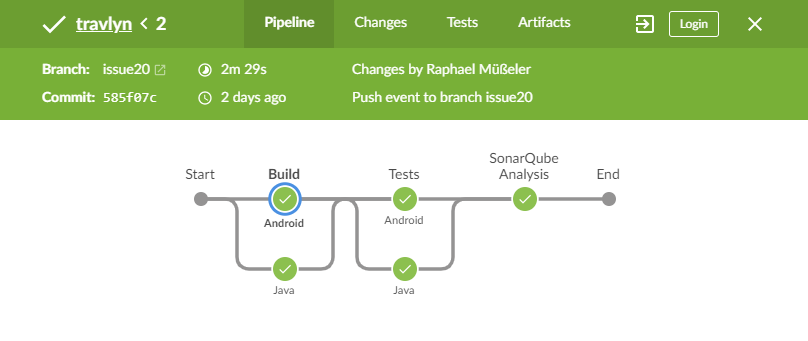
\includegraphics[width=1\textwidth]{images/jenkins-pipeline.png}
				\caption{Darstellung der für das Projekt \textit{Travlyn} erstellten Jenkins Pipeline}
				\label{fig:jenkinsPipeline}
			\end{figure} 
		
			\autoref{fig:jenkinsPipeline} zeigt die für diese Arbeit erstellte Pipeline. Die Abbildung besteht aus drei Schritten: Zunächst werden Frontend und Backend kompiliert. So können Syntax- und Kompilierfehler erkannt werden. Im darauffolgenden Schritt werden die sich sowohl im Frontend als auch im Backend befindlichen Tests ausgeführt. Anschließend die Analyse der Code Qualität mittels SonarQube (siehe \autoref{qm.sonarqube}) durchgeführt. 
		
		\subsection{Continuous Delivery}
		
			\ac{CD} bezeichnet die kontinuierliche und im Besonderen automatisierte Auslieferung einer Applikation. Ziel ist, dass, nachdem ein Build die Pipeline erfolgreich durchlaufen hat, der Build Server -- z.B. Jenkins -- Artefakte der Applikation speichert und zur Verfügung stellt. Diese Artefakte sind häufig das Kompilat der Applikation, die sich Kunden und Nutzer herunterladen können. Artefakte können aber ebenso gut Docker Images sein, mit deren Hilfe der Auslieferungsprozess simplifiziert wird. \cite{Humble.2011}
		                                                                                                                                                                                                                                                                                                                                         
	